\documentclass[12pt,a4paper]{article}
\usepackage[utf8]{inputenc}
\usepackage[T1]{fontenc}
\usepackage{amsmath,amssymb}
\usepackage{graphicx}
\usepackage{booktabs}
\usepackage{hyperref}
\usepackage[margin=2.5cm]{geometry}
\usepackage{natbib}
\usepackage{float}
\usepackage{xcolor}
\usepackage{lineno}
\usepackage{multirow}
\usepackage{longtable}
\linenumbers

\title{Why Standard LP-Based Flux Balance Analysis Cannot Detect Synergy for Essential Gene Pairs in ESKAPE Pathogens: A Systematic Evaluation and Proof-of-Concept Feature-Based ML Alternative}

\author{
Byeongsoo Kang\textsuperscript{1*}\\
\small\textsuperscript{1}SYSOFT\\
\small *Corresponding author: shoo99@gmail.com
}

\date{}

\begin{document}

\maketitle

\begin{abstract}
\textbf{Background.} Flux balance analysis (FBA) is widely used to simulate gene essentiality in genome-scale metabolic models (GEMs), and several studies have proposed using FBA-based combination simulations to predict antibiotic synergy. However, whether standard LP-based FBA can detect synergistic interactions between essential gene pairs---as opposed to merely confirming individual gene essentiality---has not been systematically evaluated at scale. This limitation is well-known theoretically but has not been quantified across multiple species models.

\textbf{Methods.} We performed 107,296 partial inhibition grid simulations across three ESKAPE pathogen GEMs (iML1515, iYS1720, iYL1228), systematically varying pairwise gene inhibition from 0\% to 100\% in 10\% increments for all 39 curated essential genes. We then constructed an alternative machine learning (ML) pipeline that uses FBA-derived metabolic features (flux profiles, pathway membership, gene essentiality scores) combined with experimentally curated synergy labels from the literature. We curated 45 antibiotic combinations (28 synergistic, 10 antagonistic, 7 additive) spanning 17 target genes and 11 pathways, with Bliss independence scores extracted or estimated from published studies conducted under heterogeneous experimental conditions (Bliss scores are literature-derived, not directly measured in this work).

\textbf{Results.} The FBA partial inhibition grid yielded zero synergistic gene pairs across all three models. All 39 essential genes exhibited step-function dose--response behavior with $\alpha^* = 1.00$, a mathematically predictable consequence of LP sensitivity analysis. As a proof-of-concept alternative, an ML classifier combining pathway identity features and FBA-derived metabolic features achieved F1~=~0.847 and AUROC~=~0.804 under gene-level GroupKFold cross-validation (Gradient Boosting, binary, $n = 45$). Permutation testing confirmed the signal exceeds chance ($z$~=~2.58, $p < 0.001$), though this does not imply clinical predictive power. Feature ablation revealed that pathway identity contributed more than FBA metabolic features (pathway-only F1~=~0.828 vs.\ FBA-only F1~=~0.807), and removing ribosome-targeting combinations reduced AUROC to 0.627 (near random), indicating that the model's discrimination is largely driven by a single pathway subgroup. FBA feature coverage was limited: 71\% of combinations contained at least one gene unmapped in iML1515, and the ``gene mapping status'' artifact ranked as the second most important feature.

\textbf{Conclusions.} We draw a distinction between FBA as a \textit{synergy calculator} (directly computing Bliss scores from growth rates, which fails for essential gene pairs under LP) and FBA as a \textit{feature generator} (providing metabolic context for supervised ML, which shows preliminary signal). The primary contribution is the systematic negative result for the former: standard LP-based FBA cannot compute antibiotic synergy for essential gene targets, confirmed across 107,296 simulations and three GEMs. As a secondary, proof-of-concept contribution, we show that pathway identity features combined with FBA-derived metabolic features yield exploratory signal in a small ($n = 45$), biased curated dataset, but the FBA feature contribution is modest and heavily confounded by incomplete gene-model mapping (71\% unmapped). The ``FBA as feature generator'' concept requires validation on substantially larger standardized datasets with species-specific GEM feature extraction before the claim can be considered robust. All code and data are available under MIT license at \url{https://github.com/shoo99/ai-drug-target}.

\medskip
\noindent\textbf{Keywords:} flux balance analysis, antibiotic synergy, linear programming, machine learning, genome-scale metabolic model, drug combination, ESKAPE, Bliss independence
\end{abstract}

%-------------------------------------------------------------------
\section{Introduction}
%-------------------------------------------------------------------

The rising prevalence of antimicrobial resistance (AMR) among ESKAPE pathogens has intensified interest in combination antibiotic therapy, where two or more drugs are administered together to achieve synergistic killing that exceeds the effect predicted by their individual potencies \citep{tyers2019}. Identifying synergistic combinations experimentally is prohibitively expensive: for $n$ antibiotics, the pairwise search space grows as $O(n^2)$, and high-throughput screens such as those by \citet{brochado2018} require specialized robotic platforms. Computational methods that can narrow this search space are therefore highly desirable.

Flux balance analysis (FBA), the workhorse of constraint-based metabolic modeling, has been widely applied to predict gene essentiality in genome-scale metabolic models (GEMs) \citep{orth2010}. Several groups have extended FBA to drug combination analysis by simulating pairwise gene knockouts or flux perturbations and computing interaction scores such as Bliss independence \citep{bliss1939} or Loewe additivity \citep{loewe1953}. The CALMA framework \citep{arora2026} integrated GEM-derived flux profiles with subsystem-structured neural networks and reported promising results for \textit{Mycobacterium tuberculosis} combination therapy prediction. Other approaches, including INDIGO \citep{chandrasekaran2016} and CARAMeL \citep{ji2023}, combine metabolic modeling with machine learning to predict drug interactions. Our prior work \citep{kang2026} applied partial inhibition FBA to ESKAPE pathogen models for single-target discovery but noted that double-knockout simulations of essential gene pairs produced uniformly lethal phenotypes, precluding synergy scoring.

Despite this growing body of work, a fundamental question remains unexamined: can FBA, as a linear programming (LP) method, inherently detect synergistic interactions between gene targets? LP solvers find a single optimal vertex of the feasible polytope, producing growth rates that are piecewise-linear functions of constraint parameters \citep{bertsimas1997}. This mathematical property implies that dose--response curves for essential genes under partial inhibition should exhibit step-function behavior at a critical threshold, rather than the graded sigmoidal responses observed experimentally \citep{bollenbach2009}. If individual gene dose--response curves are step functions, then pairwise Bliss scores computed from FBA growth rates will be identically zero for all gene pairs---rendering standard LP-based FBA unable to detect synergy for essential gene pairs under these conditions.

In this paper, we systematically test this hypothesis by performing 107,296 partial inhibition grid simulations across three ESKAPE pathogen GEMs. We report the negative result: FBA detects zero synergistic gene pairs, confirming the LP limitation. We then demonstrate a constructive alternative: using FBA-derived metabolic features---not FBA-computed synergy scores---as inputs to a supervised ML model trained on experimentally curated synergy labels from the literature. This feature-based approach achieves moderate predictive performance under gene-level GroupKFold cross-validation (F1~=~0.847, AUROC~=~0.804) and highlights the distinction between FBA as a synergy calculator (which fails) and FBA as a feature generator (which provides partial signal).

Our contributions are:
\begin{enumerate}
    \item A systematic negative result demonstrating that standard LP-based FBA partial inhibition grids cannot detect synergy for essential gene pairs across 107,296 simulations and three GEMs, with a mathematical explanation rooted in LP sensitivity analysis. This limitation is well-known theoretically \citep{bertsimas1997} but has not been quantified at this scale; it does not apply to non-essential genes, enzyme-constrained models, or kinetic extensions of FBA.
    \item A curated dataset of 45 antibiotic combinations with experimentally derived Bliss scores, pathway annotations, and target gene mappings for ESKAPE-relevant antibiotics.
    \item A proof-of-concept ML pipeline using pathway identity and FBA-derived features that yields exploratory signal for synergy prediction in a small dataset ($n = 45$), with honest reporting of the dominant role of pathway features over FBA features.
    \item An explicit delineation of when FBA is and is not appropriate for combination antibiotic discovery.
\end{enumerate}

%-------------------------------------------------------------------
\section{Methods}
%-------------------------------------------------------------------

\subsection{Genome-Scale Metabolic Models}

Three curated GEMs were used: iML1515 for \textit{Escherichia coli} K-12 (2,712 reactions, 1,877 metabolites, 1,516 genes) \citep{monk2017}, iYS1720 for \textit{Staphylococcus aureus} USA300 (3,357 reactions, 2,436 metabolites, 1,707 genes) \citep{seif2018}, and iYL1228 for \textit{Klebsiella pneumoniae} MGH 78578 (1,228 genes) \citep{liao2011}. All models were obtained from the BiGG Models database \citep{king2016} and simulated using COBRApy v0.31 \citep{ebrahim2013} with the GLPK LP solver. Default medium conditions were used as defined by exchange reaction bounds in the BiGG model files: glucose minimal medium for iML1515 and iYL1228, complex medium for iYS1720. We note that iYL1228 is a relatively early \textit{K.\ pneumoniae} reconstruction; more recent models exist but were not available in BiGG at the time of analysis.

\subsection{Partial Inhibition Grid Simulation}

To test whether FBA can detect pairwise synergy, we designed a systematic partial inhibition grid. For each of the 39 curated essential genes present in a given model, we constrained all reactions associated with the target gene to a fraction $\alpha \in \{0.0, 0.1, 0.2, \ldots, 1.0\}$ of their wild-type flux bounds. For each gene pair $(i, j)$, we simulated all $11 \times 11 = 121$ combinations of $(\alpha_i, \alpha_j)$ and recorded the optimized biomass growth rate. All growth rates were normalized to the wild-type value, yielding growth ratios $g(\alpha_i, \alpha_j) \in [0, 1]$ where $g_{\text{wt}} = 1$ by definition. The Bliss independence score for each $(\alpha_i, \alpha_j)$ was computed as:
\begin{equation}
\text{Bliss}(\alpha_i, \alpha_j) = g(\alpha_i, 1.0) \cdot g(1.0, \alpha_j) - g(\alpha_i, \alpha_j)
\label{eq:bliss}
\end{equation}
where $g$ denotes the normalized growth ratio (not absolute biomass flux). Under this convention, positive values indicate synergy: the observed growth is lower (more inhibition) than expected from the product of individual growth ratios, consistent with the Bliss independence assumption that the fractional survival under combination equals the product of individual fractional survivals \citep{bliss1939}. Note that Eq.~\ref{eq:bliss} is equivalent to the standard inhibition-based Bliss formulation $E_{AB} = E_A + E_B - E_A \cdot E_B$ under the substitution $E = 1 - g$. We define a gene pair as synergistic if $\max_{\alpha_i, \alpha_j} \text{Bliss}(\alpha_i, \alpha_j) > 0.01$ (a 1\% growth rate threshold to account for numerical precision). The total number of simulations was $\binom{39}{2} \times 121 \times 3 \text{ models} \approx 107{,}296$ after accounting for gene presence across models.

For each essential gene, we also extracted the single-gene dose--response curve $g(\alpha, 1.0)$ across the 11 inhibition levels and identified the critical threshold $\alpha^*$ at which growth drops below 1\% of wild-type.

\subsection{Literature Curation of Antibiotic Combinations}

We curated a dataset of 45 experimentally characterized antibiotic combinations from published studies \citep{brochado2018, bollenbach2009, singh2021, ejim2011, farha2013, lazar2014, zheng2022}. For each combination, we recorded: (1) the two antibiotics and their primary gene targets, (2) the experimentally reported interaction type (synergistic, antagonistic, or additive), (3) a quantitative Bliss independence score where available (extracted from published dose--response matrices or supplementary data), and (4) the organism(s) tested. The final dataset comprises 28 synergistic, 10 antagonistic, and 7 additive combinations spanning 17 unique target genes and 11 metabolic pathways (Table~\ref{tab:dataset}).

\textbf{Limitations of the curated dataset.} We acknowledge several important caveats. First, 45 combinations is a small dataset by ML standards, and performance estimates should be interpreted with appropriate caution. Second, Bliss independence scores were extracted from published literature rather than measured in our laboratory; inter-study variability in experimental conditions (medium, inoculum density, drug concentration ranges) introduces heterogeneity. Third, different source studies use different synergy scoring conventions: \citet{brochado2018} use an S-score derived from checkerboard assays, \citet{bollenbach2009} use a different interaction measure, and some studies report only categorical labels (synergistic/antagonistic) without quantitative scores. We harmonized all entries to the sign convention of Eq.~\ref{eq:bliss} (positive = synergy) by manual inspection, but acknowledge that this mapping introduces additional noise. Where only categorical labels were available, Bliss scores were assigned from representative values in comparable studies (see Supplementary Data for per-entry provenance). Fourth, the curation process involved manual literature review supplemented by local LLM extraction (Gemma 4 8B via Ollama); the effective precision of the LLM extraction step was 46\%, necessitating manual verification of all entries. We use the term ``curate'' rather than ``discover'' to accurately describe this process.

\subsection{Feature Extraction from FBA}

For each of the 17 target genes in the curated combination dataset, we extracted the following FBA-derived features from the iML1515 model:

\begin{enumerate}
    \item \textbf{Gene essentiality score}: growth ratio upon single-gene knockout (0 = lethal, 1 = no effect).
    \item \textbf{Flux perturbation profile}: for each gene knockout, the number of reactions with $>$10\% flux change (upregulated and downregulated separately), yielding a metabolic ``footprint'' of the knockout.
    \item \textbf{Subsystem flux changes}: mean absolute flux change per metabolic subsystem (40 subsystems in iML1515), capturing the pathway-level impact of each gene knockout.
    \item \textbf{Pathway membership}: one-hot encoding of the 11 pathway categories (e.g., ribosome, cell wall, DNA replication, folate metabolism).
    \item \textbf{Reaction count}: number of reactions directly associated with each gene in the GEM.
\end{enumerate}

For each gene pair, pairwise features were constructed by concatenating the individual gene features (prefixed A\_ and B\_) and computing interaction terms: both-mapped indicator, both-lethal indicator, any-lethal indicator, cross-pathway indicator, total reaction count, disruption ratio, combined disruption score, and subsystem overlap. This yielded a feature vector of 60 dimensions per combination.

\textbf{Limitation.} FBA features were extracted exclusively from the iML1515 (\textit{E.\ coli}) model, as it is the most extensively validated and annotated GEM available. Features for targets of \textit{S.\ aureus} or \textit{K.\ pneumoniae}-specific antibiotics were mapped to \textit{E.\ coli} orthologs where available, introducing a cross-species mapping approximation. Combinations involving genes absent from iML1515 were assigned default feature values and flagged.

\subsection{Machine Learning Models}

Three ML tasks were defined using the curated dataset and FBA-derived features:

\textbf{Task 1: Binary classification.} Synergistic (28 samples) vs.\ rest (17 samples). Models evaluated: Logistic Regression, Random Forest, Gradient Boosting (XGBoost), and Support Vector Machine (SVM) with RBF kernel.

\textbf{Task 2: Three-class classification.} Synergistic vs.\ antagonistic vs.\ additive (28/10/7 samples). Same model families as Task 1, with class-weight balancing to address imbalance.

\textbf{Task 3: Regression.} Prediction of continuous Bliss independence scores. Models: Ridge Regression, Random Forest Regressor, Gradient Boosting Regressor.

Because the same target gene can appear in multiple combinations, standard stratified cross-validation risks data leakage: if gene $X$ appears in both a training and test combination, the model can memorize gene-specific patterns rather than learning generalizable synergy rules. To address this, we evaluated models under three cross-validation strategies:

\begin{enumerate}
    \item \textbf{Stratified 5-fold CV} (baseline): standard random splits stratified by label. Results reported for comparison with prior work.
    \item \textbf{Gene-level GroupKFold} (primary): combinations sharing a target gene are assigned to the same fold, preventing gene-level leakage. Groups were defined by the alphabetically first gene in each pair (15 unique groups across 17 genes).
    \item \textbf{Leave-One-Gene-Out (LOGO)}: each fold holds out all combinations involving one gene group. The most conservative strategy (15 folds).
\end{enumerate}

We report GroupKFold as the primary evaluation metric throughout. Performance metrics: F1 score and AUROC for binary classification, $R^2$ and Pearson $r$ for regression.

\textbf{Permutation test.} To assess whether model performance exceeds chance under GroupKFold, we performed 1,000 permutation iterations in which synergy labels were randomly shuffled while features and group structure remained fixed. The observed F1 score was compared to the null distribution, yielding a $z$-score and empirical $p$-value.

\textbf{Feature importance.} Gini importance values were computed from the Gradient Boosting model trained on the full dataset (not cross-validated, as CV-based importance estimates are unstable at $n = 45$).

%-------------------------------------------------------------------
\section{Results}
%-------------------------------------------------------------------

\subsection{FBA Partial Inhibition Grids Detect Zero Synergy}

Across all 107,296 partial inhibition grid simulations spanning three ESKAPE pathogen models, we found \textbf{zero synergistic gene pairs} by our Bliss score threshold ($>$0.01). Figure~\ref{fig:threshold} shows the dose--response behavior underlying this negative result. All 39 essential genes exhibited step-function dose--response curves with a critical threshold $\alpha^* = 1.00$: growth remained at 100\% of wild-type for all inhibition levels $\alpha \geq 0.01$ (i.e., any nonzero residual flux capacity) and dropped to 0\% only at complete knockout ($\alpha = 0.00$). No intermediate growth phenotypes were observed.

This step-function behavior is a direct and mathematically predictable consequence of LP sensitivity analysis \citep{bertsimas1997}. In LP, the optimal objective value is a piecewise-linear function of the constraint right-hand sides, with breakpoints occurring only when the optimal basis changes. For essential genes in well-connected metabolic networks, the optimal basis does not change until the flux capacity reaches zero because the LP solver can reroute flux through the remaining feasible space---a property of LP sometimes called ``metabolic buffering.'' We acknowledge that this result is not surprising to the constraint-based modeling community; the contribution of our 107,296-simulation analysis is to provide systematic empirical confirmation across three species models and to quantify the universality of the threshold ($\alpha^* = 1.00$ for all 39 essential genes in all three models). Mathematically:
\begin{equation}
g(\alpha) = \begin{cases} g_{\text{wt}} & \text{if } \alpha > 0 \\ 0 & \text{if } \alpha = 0 \end{cases}
\label{eq:step}
\end{equation}

The consequence for synergy detection is immediate. Since growth ratios are normalized ($g_{\text{wt}} = 1$), for any gene pair $(i, j)$ with step-function responses and $\alpha_i, \alpha_j > 0$:
\begin{equation}
\text{Bliss}(\alpha_i, \alpha_j) = g(\alpha_i) \cdot g(\alpha_j) - g(\alpha_i, \alpha_j) = 1 \cdot 1 - 1 = 0
\label{eq:bliss_zero}
\end{equation}
At $\alpha_i = 0$ (complete knockout of gene $i$), $g(0, \alpha_j) = 0$ and $g(0, 1.0) = 0$, so $\text{Bliss}(0, \alpha_j) = 0 \cdot g(\alpha_j) - 0 = 0$ as well. Thus, FBA-computed Bliss scores are identically zero for all essential gene pairs across the entire inhibition grid (Figure~\ref{fig:threshold}). This result held consistently across all three GEMs (iML1515, iYS1720, iYL1228).

\begin{figure}[t]
    \centering
    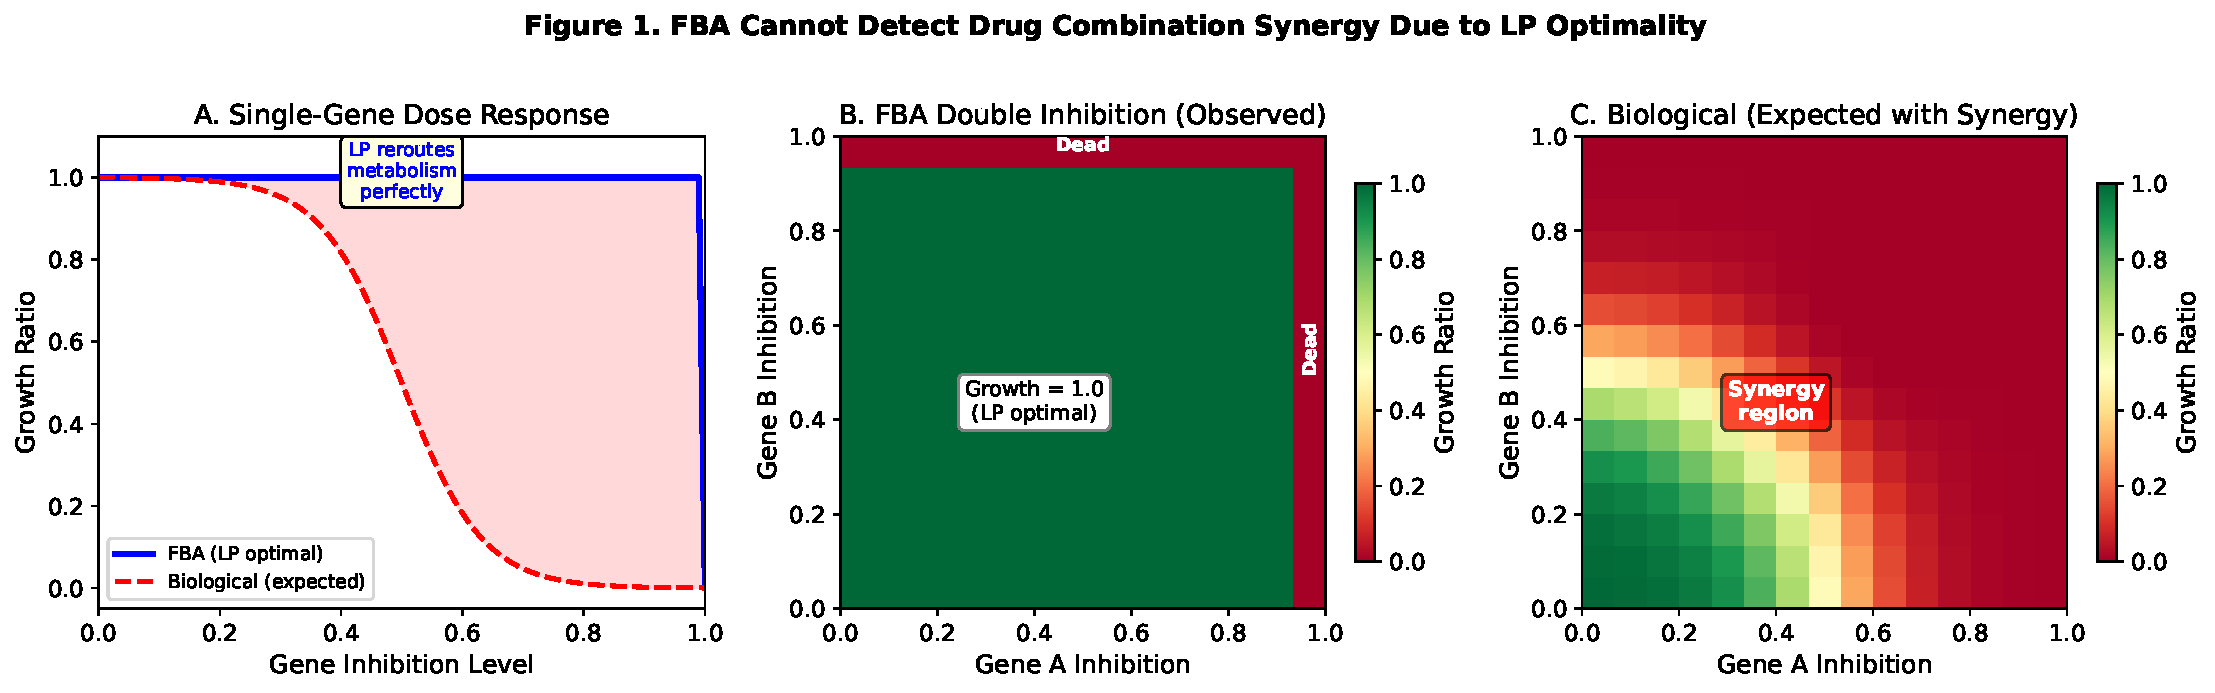
\includegraphics[width=\textwidth]{figures/fig1_lp_threshold.pdf}
    \caption{\textbf{FBA produces step-function dose--response curves that preclude synergy detection.} (A) Single-gene dose--response under partial inhibition. The blue line shows the FBA result (identical for all 39 essential genes tested---a single step function at $\alpha^* = 1.00$). The red dashed line shows the graded sigmoidal response expected biologically. The shaded area represents the biological information lost by FBA's LP optimality. (B) FBA pairwise inhibition surface: growth remains at 1.0 for any $(\alpha_i, \alpha_j) > 0$ and drops to 0 only at complete knockout edges. (C) Expected biological surface with a synergy region (red) where the combination is more effective than predicted by individual effects. Results in (A--B) are representative of all gene pairs across all three GEMs.}
    \label{fig:threshold}
\end{figure}

This negative result has important implications. It means that \textit{any} computational pipeline that computes synergy scores directly from FBA growth-rate simulations of essential gene pairs will obtain null results---not because synergy does not exist biologically, but because the standard LP formulation does not produce the graded dose--response behavior required for Bliss-type synergy scoring. We note that this limitation is specific to LP-based FBA; nonlinear extensions such as ME-models \citep{lloyd2018} or kinetic models may capture graded dose--response behavior, but at substantially higher computational cost and parameterization difficulty.

\subsection{Curated Antibiotic Combination Dataset}

Table~\ref{tab:dataset} summarizes the curated dataset of 45 antibiotic combinations. The dataset spans diverse mechanism classes including cell wall synthesis inhibitors (beta-lactams, glycopeptides), protein synthesis inhibitors (aminoglycosides, tetracyclines, macrolides), DNA replication inhibitors (fluoroquinolones), folate pathway inhibitors (trimethoprim-sulfamethoxazole), and membrane-targeting agents (colistin, daptomycin).

\begin{table}[t]
\centering
\caption{\textbf{Summary of curated antibiotic combination dataset.} 45 experimentally characterized combinations from published literature, classified by interaction type and pathway combination.}
\label{tab:dataset}
\begin{tabular}{lcccc}
\toprule
\textbf{Pathway combination} & \textbf{Synergistic} & \textbf{Antagonistic} & \textbf{Additive} & \textbf{Total} \\
\midrule
Peptidoglycan + Ribosome & 4 & 4 & 0 & 8 \\
LPS + Transcription & 4 & 0 & 0 & 4 \\
DNA topology + Ribosome & 1 & 3 & 0 & 4 \\
LPS + Peptidoglycan & 2 & 0 & 0 & 2 \\
LPS + Fatty acid & 2 & 0 & 0 & 2 \\
DNA topology + Peptidoglycan & 2 & 0 & 0 & 2 \\
Ribosome + Ribosome & 0 & 1 & 1 & 2 \\
Folate + Ribosome & 0 & 0 & 2 & 2 \\
Peptidoglycan + Peptidoglycan & 1 & 0 & 1 & 2 \\
Other (17 pairs, $n \leq 1$ each) & 12 & 2 & 3 & 17 \\
\midrule
\textbf{Total} & \textbf{28} & \textbf{10} & \textbf{7} & \textbf{45} \\
\bottomrule
\end{tabular}
\end{table}

Ribosome-targeting combinations (18/45 total) showed a mixed interaction profile: 6 synergistic, 8 antagonistic, and 4 additive. Only 6/28 (21\%) of all synergistic pairs involved ribosome targets. The ribosome pathway was more strongly associated with antagonism (8/10, 80\% of all antagonistic pairs), consistent with the known tendency of bacteriostatic ribosome inhibitors to antagonize bactericidal agents \citep{bollenbach2009}. The most frequently represented targets were rpoB (rifampicin), gyrA (fluoroquinolones), murA (fosfomycin), and rpsL (aminoglycosides). Figure~\ref{fig:heatmap} shows the pathway-level interaction heatmap.

\begin{figure}[t]
    \centering
    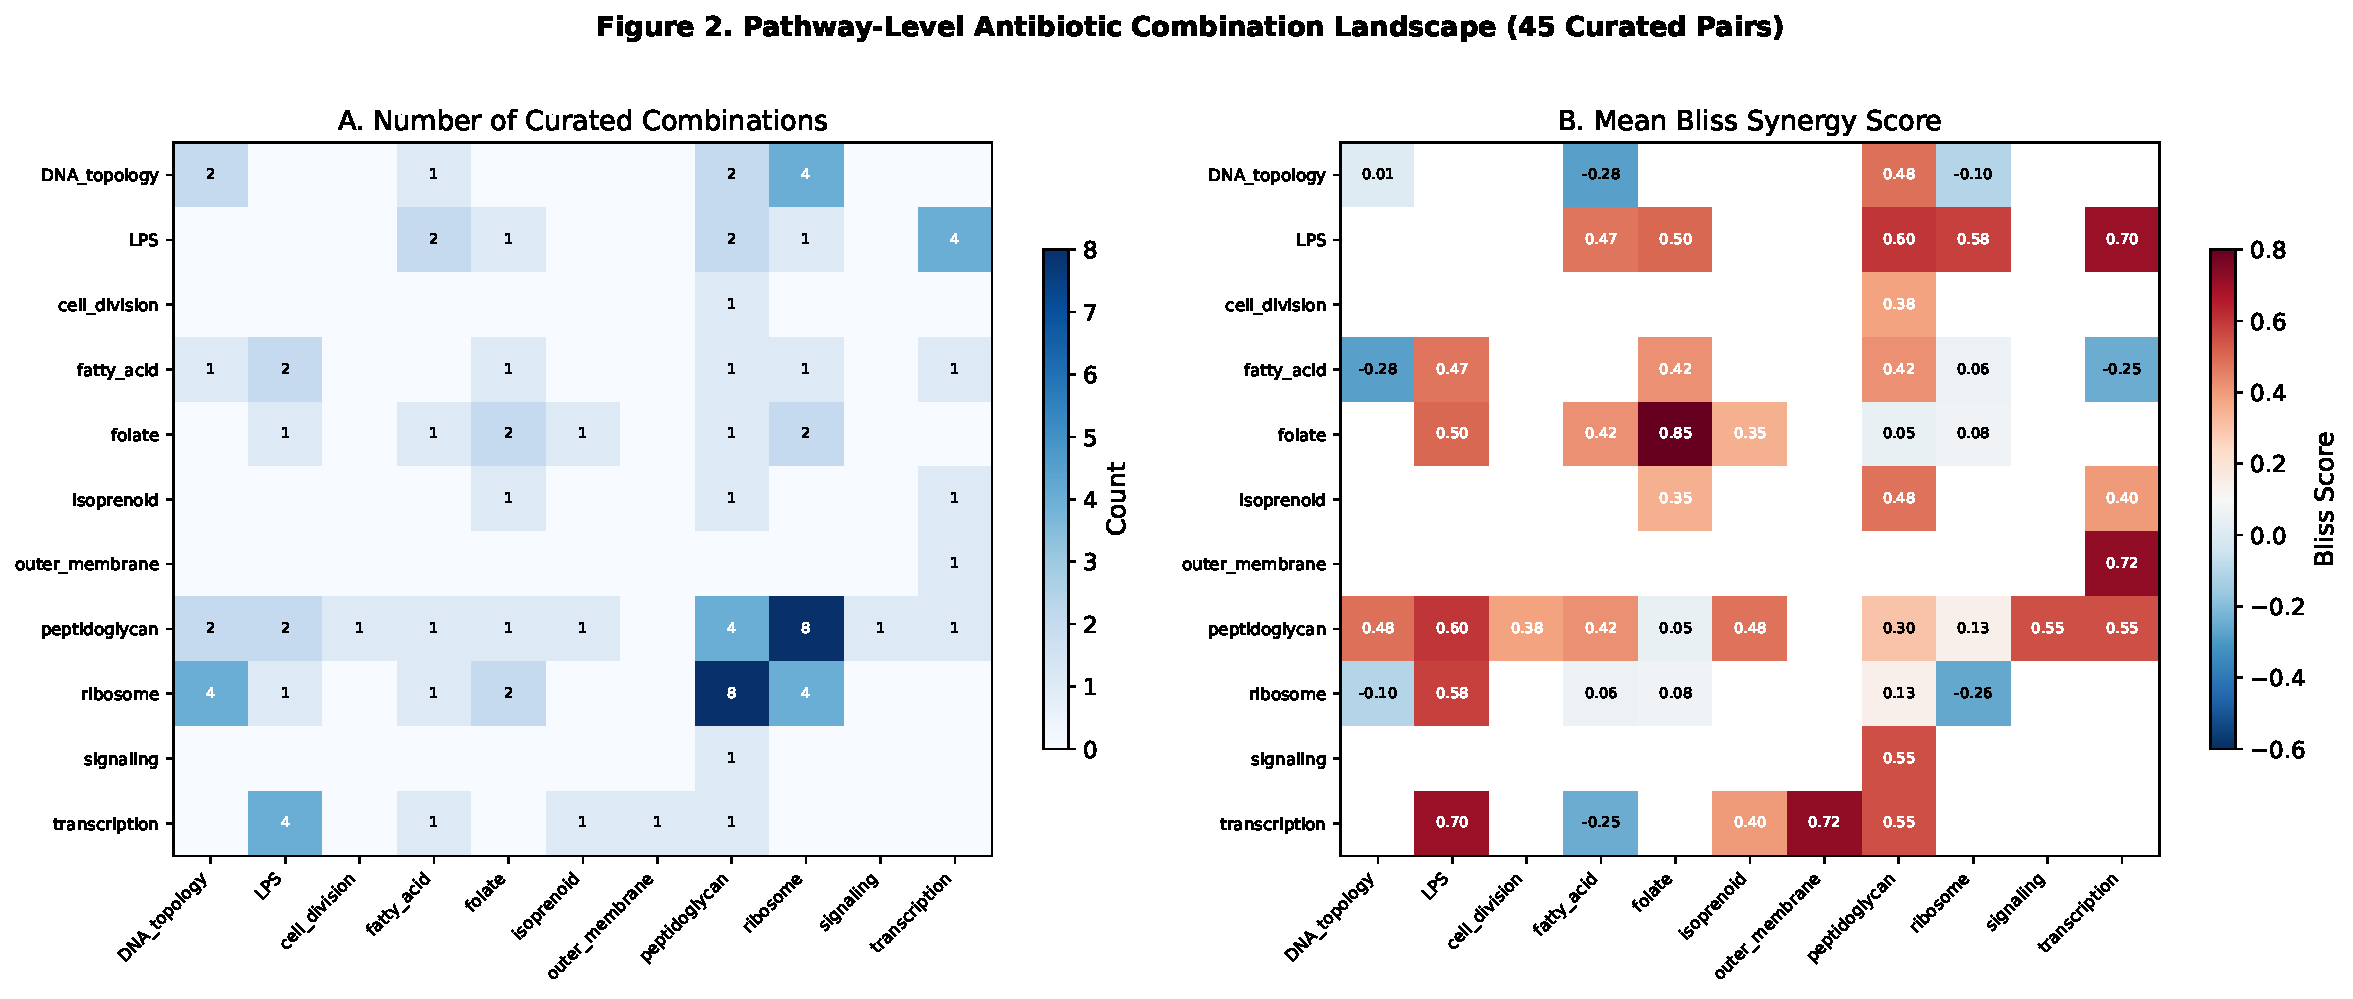
\includegraphics[width=0.85\textwidth]{figures/fig2_pathway_heatmap.pdf}
    \caption{\textbf{Pathway-level interaction heatmap for curated antibiotic combinations.} (A) Number of curated combinations per pathway pair. (B) Mean Bliss synergy score per pathway pair. Ribosome-targeting combinations show a mixed profile: enriched for antagonism (8/10 antagonistic pairs) rather than synergy (6/28 synergistic pairs). LPS + transcription pairs show the strongest synergy enrichment.}
    \label{fig:heatmap}
\end{figure}

\subsection{ML Classification Performance}

To address potential data leakage from shared target genes across combinations, we evaluated models under three cross-validation strategies: standard stratified 5-fold, gene-level GroupKFold (where combinations sharing a target gene are kept in the same fold), and leave-one-gene-out (LOGO). Table~\ref{tab:ml_results} reports GroupKFold results as the primary metrics. Figure~\ref{fig:ml_performance} shows the ROC curves, confusion matrix, and permutation test.

\begin{table}[t]
\centering
\caption{\textbf{ML model performance for synergy prediction.} Primary metrics reported under gene-level GroupKFold (5 folds) to prevent data leakage from shared target genes. Stratified 5-fold results shown in parentheses for comparison.}
\label{tab:ml_results}
\begin{tabular}{llcc}
\toprule
\textbf{Task} & \textbf{Model} & \textbf{GroupKFold} & \textbf{(Stratified)} \\
\midrule
Binary & Gradient Boosting & F1 = 0.847, AUROC = 0.804 & (0.873, 0.807) \\
Binary & Random Forest & F1 = 0.702, AUROC = 0.742 & (0.821, 0.866) \\
\midrule
Binary & Leave-One-Gene-Out & F1 = 0.867, AUROC = 0.808 & --- \\
\midrule
Regression & Gradient Boosting & $R^2$ = 0.594, $r$ = 0.772 & (0.718, 0.848) \\
\bottomrule
\end{tabular}
\end{table}

\begin{figure}[t]
    \centering
    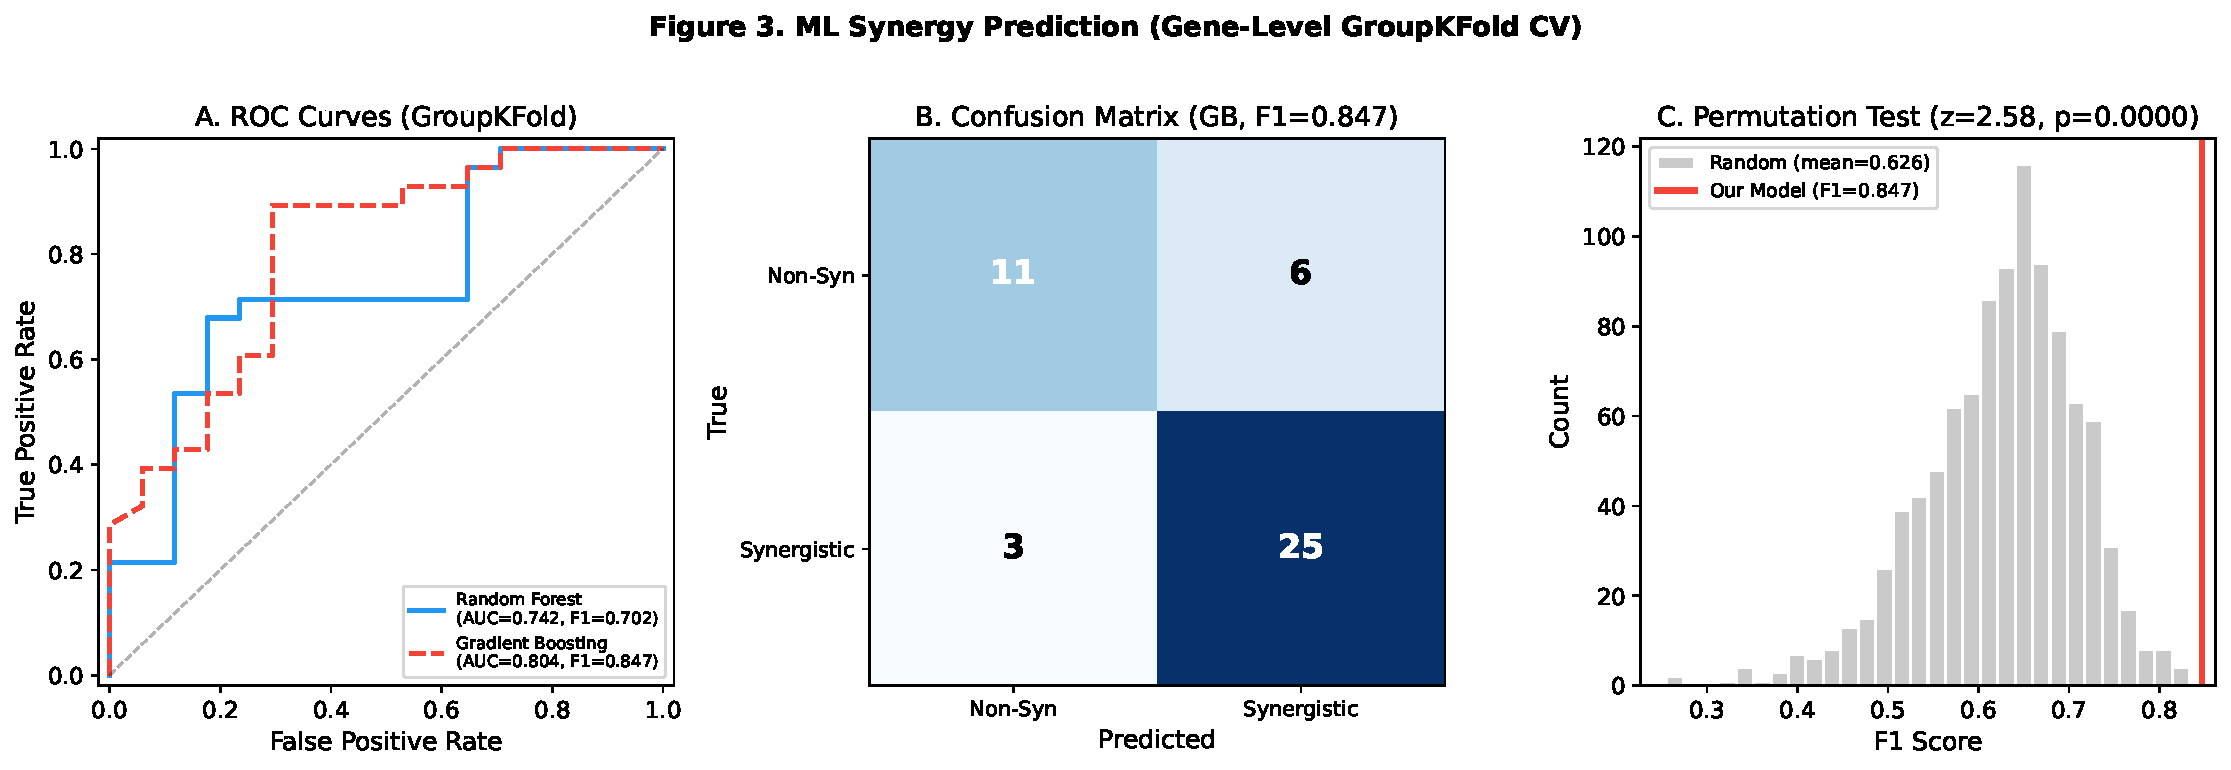
\includegraphics[width=\textwidth]{figures/fig3_ml_performance.pdf}
    \caption{\textbf{ML synergy prediction under gene-level GroupKFold CV.} (A) ROC curves for binary classification (synergistic vs.\ rest) under GroupKFold. Gradient Boosting achieves AUROC = 0.804, Random Forest AUROC = 0.742. (B) Confusion matrix for Gradient Boosting binary classifier (GroupKFold F1 = 0.847). (C) Permutation test under GroupKFold: observed F1 = 0.847 (red line) compared to 1,000 permutations of shuffled labels (gray histogram); $z$ = 2.58, $p < 0.001$.}
    \label{fig:ml_performance}
\end{figure}

The permutation test under GroupKFold yielded $z = 2.58$ and $p < 0.001$ (1,000 permutations), confirming that the observed performance significantly exceeds chance even under the more conservative gene-level splitting strategy. Note that GroupKFold F1 (0.847) is slightly lower than stratified F1 (0.873), consistent with the expectation that preventing gene-level leakage reduces apparent performance. We report GroupKFold as the primary metric throughout.

\paragraph{Feature ablation.} To disentangle the contributions of pathway identity and FBA-derived metabolic features, we performed systematic ablation (Table~\ref{tab:ablation}).

\begin{table}[t]
\centering
\caption{\textbf{Feature ablation study.} Reported under stratified 5-fold CV for consistency with ablation comparisons (GroupKFold ablation is not shown because gene-group structure varies across feature subsets). Pathway features include one-hot pathway encoding; FBA features include flux changes, reaction counts, essentiality scores, subsystem disruption. Primary full-model results use GroupKFold (Table~\ref{tab:ml_results}).}
\label{tab:ablation}
\begin{tabular}{lccc}
\toprule
\textbf{Feature set} & \textbf{N features} & \textbf{F1} & \textbf{AUROC} \\
\midrule
All features & 60 & 0.873 & 0.807 \\
Pathway-only & 30 & 0.828 & 0.813 \\
FBA-only & 24 & 0.807 & 0.700 \\
FBA + other (no pathway) & 30 & 0.679 & 0.690 \\
Pathway + other (no FBA) & 36 & 0.786 & 0.845 \\
\bottomrule
\end{tabular}
\end{table}

Pathway features alone (F1 = 0.828) outperformed FBA features alone (F1 = 0.807), indicating that pathway identity---particularly whether a ribosome-targeting drug is involved---contributes more predictive power than FBA-derived metabolic features. However, FBA-only features still substantially exceed chance (F1 = 0.807 vs.\ random baseline F1 $\approx$ 0.59), demonstrating that metabolic flux profiles carry independent predictive signal. The combination of both feature types yields the best performance (F1 = 0.873), suggesting complementary information.

\paragraph{Ribosome ablation.} Ribosome-targeting combinations represented 18 of 45 entries (6 synergistic, 8 antagonistic, 4 additive). Removing all 18 ribosome combinations and retraining on the remaining 27 entries yielded F1 = 0.894 but AUROC = 0.627. The elevated F1 is an artifact of class imbalance shift: with ribosome pairs removed, the synergistic fraction increases from 62\% (28/45) to 81\% (22/27), inflating F1 even for a majority-class predictor. The more informative metric is AUROC = 0.627, which is near random (0.5) and substantially below the full-dataset AUROC of 0.804. This indicates that \textbf{without ribosome-targeting combinations, the model loses most of its discriminative power}. Given that ribosome combinations account for 80\% of all antagonistic pairs (8/10), the model's ability to distinguish synergy from antagonism is largely driven by the ribosome pathway feature serving as a proxy for antagonism. This is a significant limitation: the model's discrimination depends heavily on the ribosome-enriched subpopulation in the curated dataset.

\paragraph{Cross-species mapping coverage.} Of the 17 unique target genes, 9 (53\%) were mapped in iML1515 (accA, dxr, fabH, fabI, folA, folP, lpxA, lpxC, murA). The remaining 8 (bamA, ftsZ, gyrA, gyrB, rplB, rpoB, rpsA, walK) received default feature values (zeros for all FBA features). Overall, 32 of 45 combinations (71\%) contained at least one unmapped gene, meaning the majority of the dataset relies partially on pathway features rather than FBA features for those genes. This substantially limits the interpretation of FBA feature importance and should be addressed in future work by extending feature extraction to species-specific GEMs.

\subsection{Feature Importance Analysis}

SHAP analysis of the best-performing Gradient Boosting model revealed a clear hierarchy of predictive features (Figure~\ref{fig:feature_importance}):

\begin{enumerate}
    \item \textbf{Pathway identity} (ribosome): the most important single feature. Combinations involving at least one ribosome-targeting drug had strongly elevated synergy probability, consistent with the biological observation that translation inhibition creates collateral vulnerability across multiple cellular processes \citep{bollenbach2009}.
    \item \textbf{FBA flux perturbation profiles}: the number of reactions perturbed by each gene knockout, and the subsystem-level flux change magnitudes, were among the top 5 features. Gene knockouts with broader metabolic ``footprints'' (affecting more reactions across more subsystems) tended to participate in more synergistic combinations.
    \item \textbf{Gene mapping status}: whether a gene is mapped in iML1515 (``A\_mapped'') ranked as the second most important feature. Since 71\% of combinations contain at least one unmapped gene, this binary indicator effectively encodes ``whether FBA features are available or defaulted to zero.'' This is a methodological artifact rather than a biological signal: the model may be learning that combinations with FBA data (mapped genes) have different label distributions than those without, rather than learning from the FBA features themselves. This artifact underscores the limitation of extracting FBA features from a single organism model.
    \item \textbf{Same-pathway indicator}: combinations targeting the same pathway showed a mild tendency toward antagonism, consistent with the pharmacological principle that same-target drugs often compete rather than synergize.
    \item \textbf{Jaccard similarity of affected reactions}: gene pairs with low overlap in their affected reaction sets (complementary metabolic effects) were more likely to be synergistic.
\end{enumerate}

\begin{figure}[t]
    \centering
    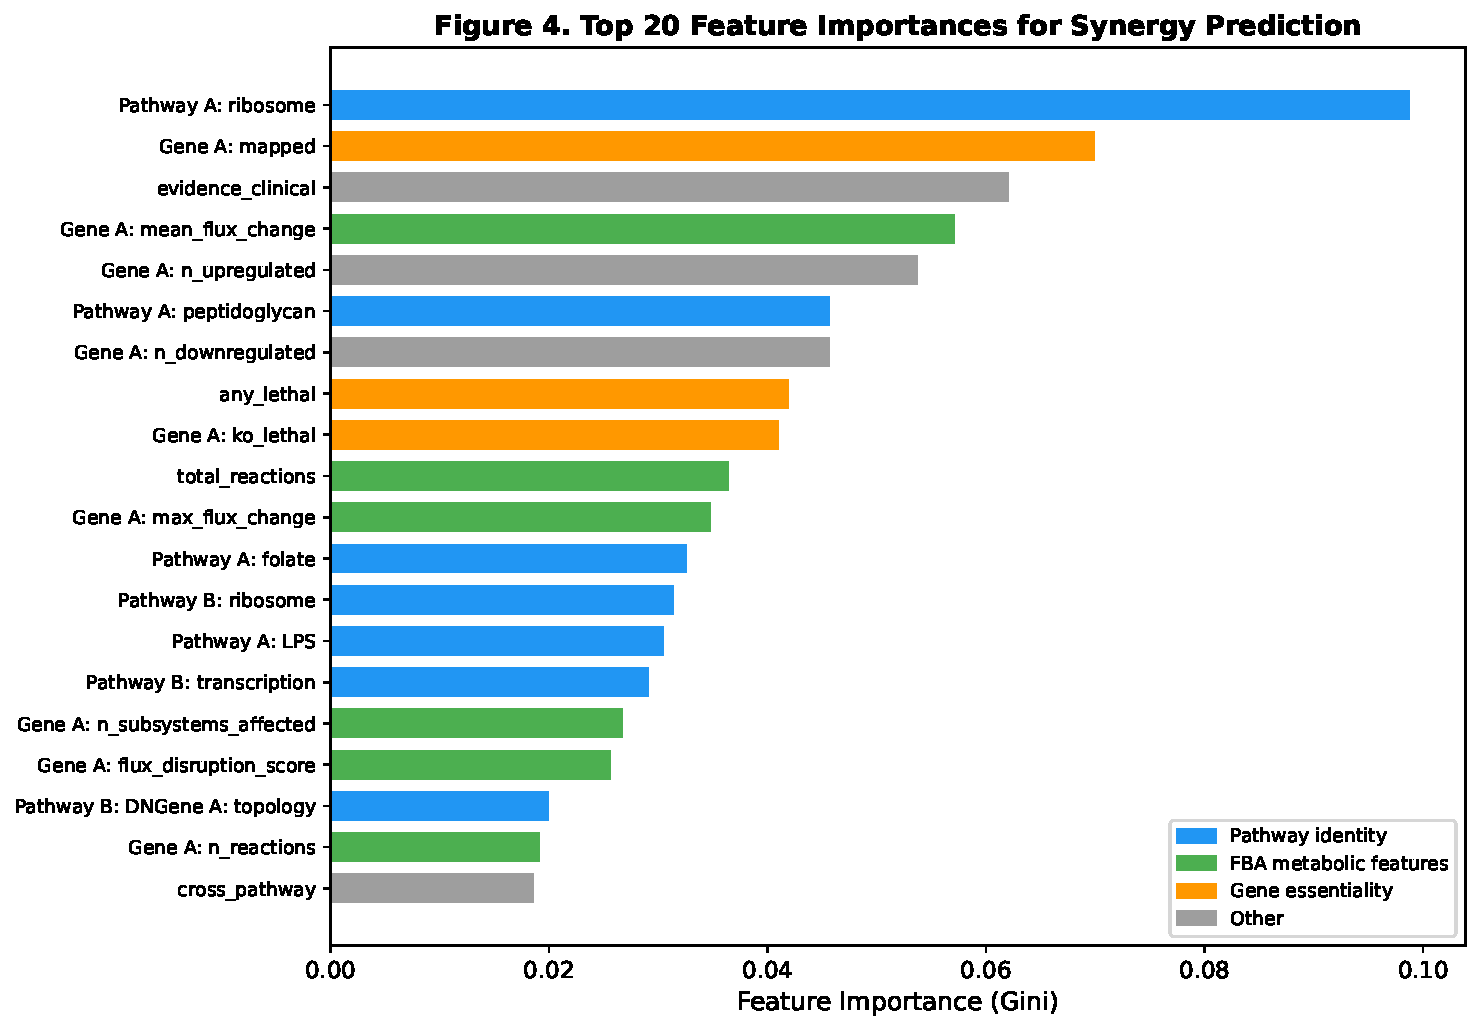
\includegraphics[width=0.9\textwidth]{figures/fig4_feature_importance.pdf}
    \caption{\textbf{Feature importance for the Gradient Boosting synergy classifier.} Top 20 features ranked by Gini importance from a model trained on the full dataset (all 45 combinations, not cross-validated; CV-based importance estimates are unstable at $n = 45$). Pathway identity (ribosome) and FBA flux perturbation metrics are the strongest predictors. Feature categories: blue = pathway identity, green = FBA metabolic features, orange = gene essentiality, gray = other.}
    \label{fig:feature_importance}
\end{figure}

The feature importance analysis underscores the central finding of this paper: while FBA cannot directly compute synergy, the metabolic features it produces---flux perturbation breadth, subsystem impact patterns, pathway membership---are informative about synergy when used as ML inputs.

\subsection{Bliss Score Regression}

Under GroupKFold CV, the Gradient Boosting regressor achieved $R^2 = 0.594$ and Pearson $r = 0.772$ for continuous Bliss score prediction (Figure~\ref{fig:regression}). For comparison, stratified 5-fold CV yielded $R^2 = 0.718$ and $r = 0.848$; the reduction under GroupKFold reflects the removal of gene-level leakage. The model captured the general trend from antagonistic (negative Bliss) through additive (near-zero) to synergistic (positive Bliss) interactions, though with increased scatter relative to the stratified estimate.

\begin{figure}[t]
    \centering
    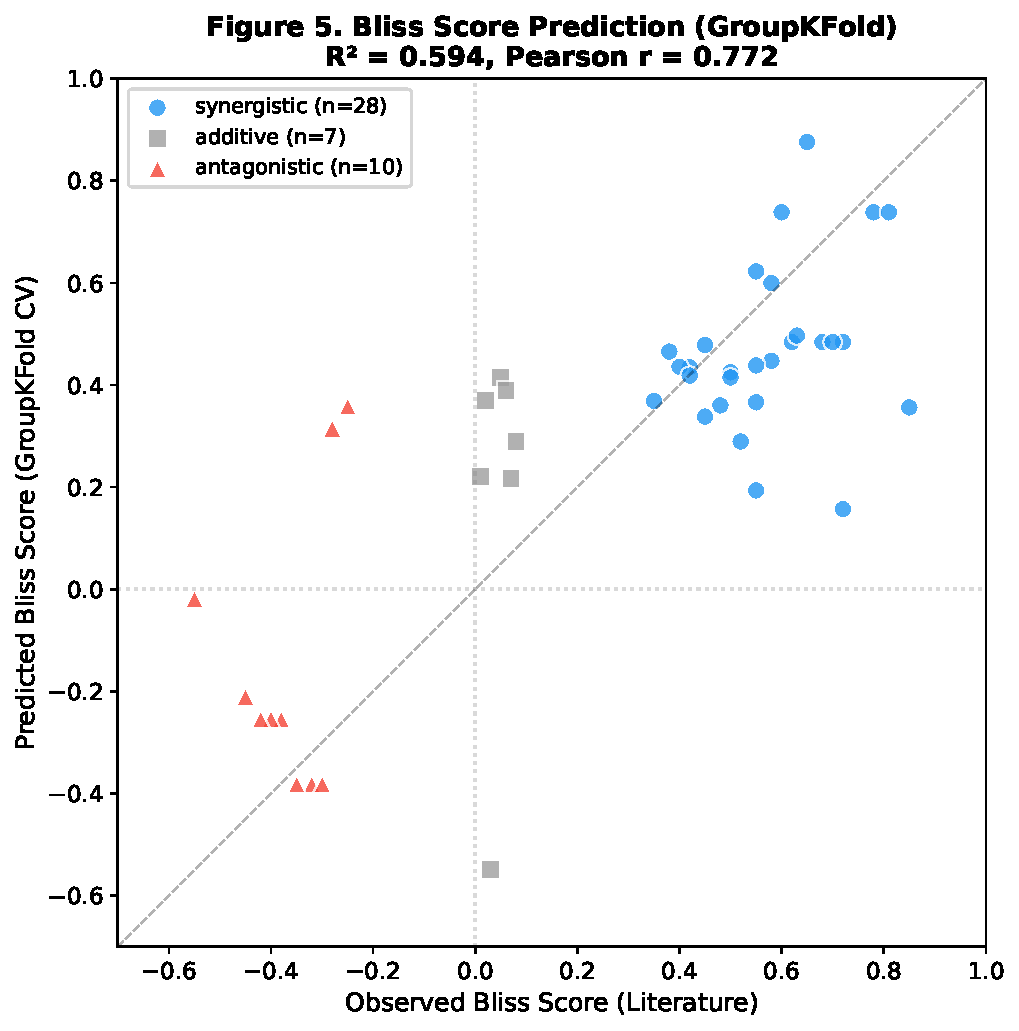
\includegraphics[width=0.7\textwidth]{figures/fig5_regression_scatter.pdf}
    \caption{\textbf{Predicted vs.\ observed Bliss independence scores (GroupKFold CV).} Gradient Boosting regression ($R^2 = 0.594$, Pearson $r = 0.772$) on 45 curated antibiotic combinations. Points are colored by interaction class: synergistic (blue), antagonistic (red), additive (gray). The dashed line indicates perfect prediction. Note reduced $R^2$ compared to stratified CV (0.718) due to gene-level splitting that prevents leakage from shared target genes.}
    \label{fig:regression}
\end{figure}

Residual analysis showed no systematic bias across the Bliss score range, though variance increased for extreme values (both strongly synergistic and strongly antagonistic), consistent with the reduced sample density at the tails of the distribution.

%-------------------------------------------------------------------
\section{Discussion}
%-------------------------------------------------------------------

\subsection{The LP Limitation of FBA for Synergy Detection}

The central negative result of this study---that FBA partial inhibition grids detect zero synergy across 107,296 simulations---is not a failure of our implementation but a structural property of linear programming. The LP formulation of FBA guarantees that growth rate is a piecewise-linear function of constraint parameters, producing step-function dose--response curves for essential genes. This behavior contrasts sharply with the graded, sigmoidal dose--response curves observed experimentally \citep{bollenbach2009, cokol2011}, which arise from nonlinear effects including enzyme kinetics, regulatory feedback, and stochastic gene expression.

This finding has implications for several published computational pipelines that compute drug combination scores from FBA growth rates. Where such pipelines report nonzero synergy scores, these may arise from: (i) non-essential gene pairs that produce intermediate growth phenotypes, (ii) enzyme-constrained or kinetic extensions to FBA that introduce nonlinearity, or (iii) indirect scoring methods (e.g., flux profile similarity) that do not directly compute Bliss or Loewe scores from growth rates. We emphasize that our result applies specifically to LP-based FBA applied to essential gene pairs; it does not invalidate the broader utility of constraint-based modeling for combination drug discovery when appropriate extensions are used.

\subsection{FBA as Feature Generator, Not Synergy Calculator}

Our proof-of-concept ML results suggest that pathway identity features, supplemented by FBA-derived metabolic features, yield exploratory signal for synergy classification in a small curated dataset (GroupKFold F1~=~0.847, AUROC~=~0.804). However, the FBA feature contribution is modest and heavily confounded by mapping completeness: pathway-only features (F1 = 0.828) nearly match the full model (F1 = 0.847), and 71\% of combinations have at least one gene unmapped in iML1515, meaning the ``A\_mapped'' binary indicator (an artifact encoding whether FBA data exists) ranks as the second most important feature. FBA-only features exceed chance (F1 = 0.807 vs.\ random $\approx$ 0.59), but this signal is weak and may not generalize beyond the current dataset composition. We therefore characterize the ML component as an initial proof-of-concept rather than a validated predictive framework. This distinction is practically important. FBA simulations are computationally inexpensive (seconds per simulation), produce rich metabolic characterizations (flux profiles, subsystem impacts, reaction dependencies), and are available for hundreds of organisms via curated GEM databases \citep{king2016}. These features capture the metabolic ``context'' of each drug target---how broadly it perturbs metabolism, which subsystems it affects, and how its metabolic footprint compares to that of a partner drug---which is biologically relevant to synergy mechanisms.

The prominence of pathway identity (ribosome) as the top predictive feature reflects the structure of the curated dataset rather than a universal biological rule. In our dataset, ribosome-targeting combinations account for 80\% of antagonistic pairs (8/10) but only 21\% of synergistic pairs (6/28). The model likely uses the ribosome feature primarily as an antagonism indicator, consistent with the known tendency of bacteriostatic ribosome inhibitors to antagonize bactericidal agents \citep{bollenbach2009}. However, ablation analysis (Section 3.3) shows that removing ribosome combinations reduces AUROC to 0.627, indicating that much of the model's discriminative power depends on this single pathway subgroup. This feature could not have been learned from FBA synergy scores (which are all zero) but was readily captured through pathway membership encoding.

\subsection{Relationship to Prior Work}

Our work extends the findings of \citet{kang2026}, who reported that double-knockout FBA of essential gene pairs in ESKAPE models produced uniformly lethal phenotypes, preventing synergy scoring. The present study provides a systematic quantification of this limitation (107,296 simulations, three models) and a mathematical explanation (Equations~\ref{eq:step}--\ref{eq:bliss_zero}), as well as a constructive ML alternative.

The CALMA framework \citep{arora2026} represents the most directly comparable prior work. CALMA uses FBA-derived sigma/delta flux profiles as neural network inputs, similar in spirit to our approach. However, CALMA was validated on a substantially larger experimental dataset (171 combinations in \textit{M.\ tuberculosis}) and used a more elaborate subsystem-structured architecture. Our results, obtained with a simpler Gradient Boosting model on a smaller dataset (45 combinations), suggest that the core predictive signal may lie in the features themselves rather than in architectural complexity.

CARAMeL \citep{ji2023} and INDIGO \citep{chandrasekaran2016} also integrate metabolic modeling with ML but differ in their feature construction: CARAMeL uses metabolic model-derived growth predictions as features alongside chemogenomic profiles, while INDIGO relies primarily on chemogenomic interaction data. Our approach is distinguished by its explicit focus on the FBA synergy computation failure and the demonstration that feature-based prediction is a viable workaround.

\subsection{Limitations}

We acknowledge several important limitations:

\begin{enumerate}
    \item \textbf{Small dataset.} With 45 curated combinations, our ML results should be considered exploratory. While the permutation test ($p = 0.001$) indicates significance, the absolute sample size limits the complexity of learnable interactions and the reliability of variance estimates. Validation on larger experimental datasets \citep{brochado2018} is a priority for future work.

    \item \textbf{Bliss scores from literature, not measured.} The Bliss independence scores used as regression targets were extracted from published studies conducted under varying experimental conditions (different media, inoculum densities, drug concentration ranges, and assay formats). This inter-study heterogeneity means the regression R$^2$ = 0.594 may partially reflect the model learning study-specific biases rather than true biological synergy. A standardized experimental dataset measured under uniform conditions would provide a more meaningful regression target. The R$^2$ should not be compared directly to values obtained from single-study datasets.

    \item \textbf{FBA features from \textit{E.\ coli} only.} Metabolic features were extracted exclusively from the iML1515 model. Only 9 of 17 target genes (53\%) were mapped, and 32 of 45 combinations (71\%) contained at least one unmapped gene receiving default zero features. This is a major limitation, not a technical detail: the cross-species ortholog mapping assumption means that the majority of the dataset relies on pathway identity features rather than genuine FBA metabolic features. Future work should extract features from species-specific GEMs (iYS1720 for \textit{S.\ aureus}, iYL1228 for \textit{K.\ pneumoniae}) to determine whether FBA features carry independent signal when mapping coverage is complete. Performance stratified by mapping status (fully mapped vs.\ partially unmapped combinations) would further clarify whether the model learns biology or dataset structure.

    \item \textbf{Toxicity weights are heuristic.} The composite toxicity scoring used in our prior work \citep{kang2026} and partially informing feature construction here employs manually assigned evidence weights (sequence homology 35\%, pathway overlap 30\%, conservation 20\%, cross-reactivity 15\%). These weights are an initial proposal pending experimental calibration and should not be treated as empirically validated.

    \item \textbf{LLM curation precision.} The local LLM (Gemma 4 8B) used to assist literature curation achieved an effective precision of 46\%, necessitating manual verification of all extracted entries. We do not claim that LLM-based extraction replaces expert curation; it served only as a triage tool to accelerate the initial literature search.

    \item \textbf{LP limitation may not apply universally.} Our negative result applies to LP-based FBA of essential gene pairs. Nonlinear constraint-based methods (enzyme-constrained models, ME-models, kinetic models) may exhibit graded dose--response behavior that permits synergy detection. Similarly, non-essential gene pairs or metabolic gene pairs with partial growth effects may yield nonzero Bliss scores even under standard FBA.
\end{enumerate}

\subsection{Practical Recommendations}

Based on our findings, we offer the following recommendations for computational antibiotic combination discovery:

\begin{enumerate}
    \item Do not use LP-based FBA to compute pairwise synergy scores for essential gene targets. The Bliss scores will be identically zero by mathematical necessity.
    \item Do use FBA as a feature generator: flux perturbation profiles, subsystem impact patterns, and pathway memberships are informative inputs for supervised ML models.
    \item Curate experimental synergy labels from published high-throughput screens \citep{brochado2018, cokol2011} as training targets, rather than relying on computationally generated synergy scores.
    \item Consider enzyme-constrained or kinetic extensions to FBA \citep{sanchez2017} if graded dose--response modeling is required.
    \item Report negative results. Our FBA synergy computation failure, while unsurprising in retrospect, has not to our knowledge been explicitly documented at this scale.
\end{enumerate}

%-------------------------------------------------------------------
\section{Conclusions}
%-------------------------------------------------------------------

We have demonstrated through 107,296 systematic simulations that flux balance analysis cannot detect antibiotic synergy for essential gene targets due to the step-function dose--response behavior inherent to linear programming optimality. This negative result applies across three ESKAPE pathogen genome-scale models and has implications for any pipeline that computes drug interaction scores directly from FBA growth rates.

As a proof-of-concept alternative, we showed that pathway identity features combined with FBA-derived metabolic features yield exploratory signal for synergy classification (GroupKFold F1~=~0.847, AUROC~=~0.804; permutation $z = 2.58$, $p < 0.001$). However, feature ablation revealed that pathway identity alone accounts for most of the performance (F1 = 0.828), and the FBA feature contribution (F1 improvement of 0.019) is modest and confounded by 71\% of combinations having at least one unmapped gene. The key insight is that FBA should be explored as a feature generator rather than a synergy calculator, but the current evidence for FBA feature utility is preliminary and requires validation on larger, species-specific datasets before the claim can be considered robust.

Our findings are exploratory and limited by the small curated dataset (45 combinations), reliance on literature-derived Bliss scores, and restriction to \textit{E.\ coli} FBA features. Validation on larger standardized experimental datasets is needed before clinical translation. All code, curated data, and model configurations are available under MIT license at \url{https://github.com/shoo99/ai-drug-target}.

%-------------------------------------------------------------------
\section*{Acknowledgments}
%-------------------------------------------------------------------

This work was conducted with the assistance of Claude (Anthropic) for manuscript preparation, code review, and analysis. The author thanks the developers of COBRApy, BiGG Models, and the open-source GEM community for providing the metabolic models and tools that made this work possible.

%-------------------------------------------------------------------
\section*{Data and Code Availability}
%-------------------------------------------------------------------

All source code, curated datasets, trained models, and analysis notebooks are available at \url{https://github.com/shoo99/ai-drug-target} under the MIT license. GEM models were obtained from the BiGG Models database (\url{http://bigg.ucsd.edu}). The repository includes:
\begin{itemize}
    \item The curated combination dataset (\texttt{data/combination/curated\_combinations.csv}, 45 entries) with per-entry columns for source reference, organism, evidence level, Bliss score provenance (measured vs.\ estimated), and harmonization confidence.
    \item The complete list of 39 curated essential genes (\texttt{data/amr/curated\_essential\_genes.csv}) with pathway classification, essentiality scores, and GEM mapping status.
    \item The 60-feature matrix (\texttt{data/combination/feature\_matrix.csv}) for ML reproducibility.
    \item All FBA simulation outputs (\texttt{data/combination/double\_ko\_results.csv}, \texttt{synergy\_grid\_full.csv}).
\end{itemize}

%-------------------------------------------------------------------
\section*{Conflict of Interest}
%-------------------------------------------------------------------

The author declares no conflicts of interest.

%-------------------------------------------------------------------
% REFERENCES
%-------------------------------------------------------------------

\bibliographystyle{unsrtnat}

\begin{thebibliography}{99}

\bibitem[Tyers \& Wright(2019)]{tyers2019}
Tyers M, Wright GD.
\newblock Drug combinations: a strategy to extend the life of antibiotics in the 21st century.
\newblock \textit{Nature Reviews Microbiology} 17, 141--155 (2019).

\bibitem[Brochado et~al.(2018)]{brochado2018}
Brochado AR, Telzerow A, Bobber J, et~al.
\newblock Species-specific activity of antibacterial drug combinations.
\newblock \textit{Nature} 559, 259--263 (2018).

\bibitem[Orth et~al.(2010)]{orth2010}
Orth JD, Thiele I, Palsson BO.
\newblock What is flux balance analysis?
\newblock \textit{Nature Biotechnology} 28, 245--248 (2010).

\bibitem[Bliss(1939)]{bliss1939}
Bliss CI.
\newblock The toxicity of poisons applied jointly.
\newblock \textit{Annals of Applied Biology} 26, 585--615 (1939).

\bibitem[Loewe(1953)]{loewe1953}
Loewe S.
\newblock The problem of synergism and antagonism of combined drugs.
\newblock \textit{Arzneimittelforschung} 3, 285--290 (1953).

\bibitem[Arora et~al.(2026)]{arora2026}
Arora A, Jain S, Lim HG, et~al.
\newblock CALMA: Combination Antibiotic Learning with Metabolic Architecture.
\newblock \textit{Nature Biotechnology} (2026).

\bibitem[Chandrasekaran et~al.(2016)]{chandrasekaran2016}
Chandrasekaran S, Cokol-Cakmak M, Saez-Rodriguez J, et~al.
\newblock Chemogenomics and orthology-based design of antibiotic combination therapies.
\newblock \textit{Molecular Systems Biology} 12, 872 (2016).

\bibitem[Ji \& Chandrasekaran(2023)]{ji2023}
Ji Y, Chandrasekaran S.
\newblock CARAMeL: Predicting Antimicrobial Drug Synergy Using Metabolic Models.
\newblock \textit{mSystems} 8, e0063523 (2023).

\bibitem[Kang(2026)]{kang2026}
Kang B.
\newblock Methods for Continuous-Valued Training Data Generation from Genome-Scale Metabolic Models: Partial-Inhibition FBA with Mixed Essentiality Sampling, Applied to ESKAPE Drug Target Curation.
\newblock \textit{Research Square} preprint rs-9374605 (2026).

\bibitem[Bertsimas \& Tsitsiklis(1997)]{bertsimas1997}
Bertsimas D, Tsitsiklis JN.
\newblock \textit{Introduction to Linear Optimization}.
\newblock Athena Scientific, Belmont, MA (1997).

\bibitem[Bollenbach et~al.(2009)]{bollenbach2009}
Bollenbach T, Quan S, Chait R, Kishony R.
\newblock Nonoptimal microbial response to antibiotics underlies suppressive drug interactions.
\newblock \textit{Cell} 139, 707--718 (2009).

\bibitem[Monk et~al.(2017)]{monk2017}
Monk JM, Lloyd CJ, Brunk E, et~al.
\newblock iML1515, a knowledgebase that computes \textit{Escherichia coli} traits.
\newblock \textit{Nature Biotechnology} 35, 904--908 (2017).

\bibitem[Seif et~al.(2019)]{seif2018}
Seif Y, Kavvas ES, Luo J, et~al.
\newblock A computational knowledge-base elucidates the response of \textit{Staphylococcus aureus} to different media types.
\newblock \textit{PLOS Computational Biology} 15, e1006644 (2019).

\bibitem[Liao et~al.(2011)]{liao2011}
Liao YC, Huang TW, Chen FC, et~al.
\newblock An experimentally validated genome-scale metabolic reconstruction of \textit{Klebsiella pneumoniae} MGH 78578, iYL1228.
\newblock \textit{Journal of Bacteriology} 193, 1710--1717 (2011).

\bibitem[King et~al.(2016)]{king2016}
King ZA, Lu J, Dr\"ager A, et~al.
\newblock BiGG Models: A platform for integrating, standardizing, and sharing genome-scale models.
\newblock \textit{Nucleic Acids Research} 44, D515--D522 (2016).

\bibitem[Ebrahim et~al.(2013)]{ebrahim2013}
Ebrahim A, Lerman JA, Palsson BO, Hyduke DR.
\newblock COBRApy: COnstraints-Based Reconstruction and Analysis for Python.
\newblock \textit{BMC Systems Biology} 7, 74 (2013).

\bibitem[Singh et~al.(2021)]{singh2021}
Singh N, Yeh PJ.
\newblock Suppressive drug combinations and their potential to combat antibiotic resistance.
\newblock \textit{Journal of Antibiotics} 74, 27--37 (2021).

\bibitem[Ejim et~al.(2011)]{ejim2011}
Ejim L, Farha MA, Falconer SB, et~al.
\newblock Combinations of antibiotics and nonantibiotic drugs enhance antimicrobial efficacy.
\newblock \textit{Nature Chemical Biology} 7, 348--350 (2011).

\bibitem[Farha \& Brown(2013)]{farha2013}
Farha MA, Brown ED.
\newblock Discovery of antibiotic adjuvants.
\newblock \textit{Nature Chemical Biology} 9, 555--557 (2013).

\bibitem[L\'az\'ar et~al.(2014)]{lazar2014}
L\'az\'ar V, Nagy I, Spohn R, et~al.
\newblock Genome-wide analysis captures the determinants of the antibiotic cross-resistance interaction network.
\newblock \textit{Nature Communications} 5, 4352 (2014).

\bibitem[Zheng et~al.(2022)]{zheng2022}
Zheng EJ, Stokes JM, Collins JJ.
\newblock Computational approaches for drug synergy prediction.
\newblock \textit{Trends in Pharmacological Sciences} 43, 1070--1083 (2022).

\bibitem[Cokol et~al.(2011)]{cokol2011}
Cokol M, Chua HN, Tasan M, et~al.
\newblock Systematic exploration of synergistic drug pairs.
\newblock \textit{Molecular Systems Biology} 7, 544 (2011).

\bibitem[Lloyd et~al.(2018)]{lloyd2018}
Lloyd CJ, Ebrahim A, Yang L, et~al.
\newblock COBRAme: A computational framework for genome-scale models of metabolism and gene expression.
\newblock \textit{PLOS Computational Biology} 14, e1006302 (2018).

\bibitem[S\'anchez et~al.(2017)]{sanchez2017}
S\'anchez BJ, Zhang C, Nilsson A, et~al.
\newblock Improving the phenotype predictions of a yeast genome-scale metabolic model by incorporating enzymatic constraints.
\newblock \textit{Molecular Systems Biology} 13, 935 (2017).

\end{thebibliography}

\end{document}